\documentclass[12pt,twoside]{report}


\usepackage[utf8]{inputenc}
\usepackage[a4paper,width=150mm,top=25mm,bottom=25mm,bindingoffset=6mm]{geometry}
\usepackage{graphicx}
\graphicspath{ {images/} }

\usepackage[backend=bibtex,style=alphabetic,sorting=none]{biblatex}
\addbibresource{tex/references.bib}

\usepackage{fancyhdr}
\pagestyle{fancy}
\rhead{}

\usepackage{float}

\usepackage{bm}
\usepackage{datetime}
\usepackage{hyperref}

\usepackage{algorithm}
\usepackage{algpseudocode}
\usepackage{amsmath}
\usepackage{amsfonts}
\usepackage{mathtools}
\usepackage{interval}

\usepackage{color}


%% Definitions %%

% ForEach loop
\algnewcommand\algorithmicforeach{\textbf{for each}}
\algdef{S}[FOR]{ForEach}[1]{\algorithmicforeach\ #1\ \algorithmicdo}

% Break
\newcommand{\Break}{\State \textbf{break} }

% Input
\algnewcommand\algorithmicinput{\textbf{Input:}}
\algnewcommand\Input{\item[\algorithmicinput]}

% Output
\algnewcommand\algorithmicoutput{\textbf{Output:}}
\algnewcommand\Output{\item[\algorithmicoutput]}

\newcommand{\R}{\mathbb{R}}  % Pretty set of real numbers.
\newcommand{\N}{\mathbb{N}}  % Pretty set of natural numbers.
\newcommand{\T}{\text{T}}  % Pretty transpose.
\newcommand{\mi}{\mathrm{i}}  % Pretty imaginary unit.
\DeclarePairedDelimiter{\ceil}{\lceil}{\rceil}  % The ceiling function.
\DeclarePairedDelimiter{\floor}{\lfloor}{\rfloor}  % The floor function.

\newcommand{\vect}[1]{\bm{\MakeLowercase{#1}}}  % Pretty vectors.
\newcommand{\mat}[1]{\mathbf{#1}}  % Pretty matrices.

\DeclareMathOperator*{\argmin}{argmin}  % Argmin
\DeclareMathOperator*{\argmax}{argmax}  % Argmax

\DeclarePairedDelimiterX{\inp}[2]{\langle}{\rangle}{#1, #2}  % Inner product

\DeclarePairedDelimiterX{\kl}[2]{\text{D}(}{)}{#1 \| #2}  % KL-Divergence
\DeclarePairedDelimiterX{\jsd}[2]{\text{JSD}(}{)}{#1 \| #2}  % JSD-Divergence

\newcommand{\doccount}{N}
\newcommand{\streamlen}{T}

\newcommand{\traj}{y}
\newcommand{\embed}{\vect{v}}

\newcommand{\featset}{\text{M}}
\newcommand{\featcount}{V}
\newcommand{\df}{DF}

\newcommand{\bowmat}{\mat{B}}  % Bag of Words matrix
\newcommand{\dtdmat}{\mat{D}}  % Document to Day matrix
\newcommand{\trajmat}{\mat{T}}  % Trajectory matrix
\newcommand{\distmat}{\mat{Dist}}  % Distance matrix

\DeclarePairedDelimiterX{\cost}[2]{\text{C}(}{)}{#1, #2}  % Cost function
\DeclarePairedDelimiterX{\trajdist}[2]{\text{Dist}(}{)}{#1, #2}  % Trajectory distance
\DeclarePairedDelimiterX{\semsim}[2]{\text{Sim}(}{)}{#1, #2}  % Semantic similarity
\DeclarePairedDelimiterX{\distfunc}[2]{\text{d}(}{)}{#1, #2}  % Distance function
\DeclarePairedDelimiterX{\kw}[1]{\text{KW}(}{)}{#1}  % Keywords representation
\DeclarePairedDelimiterX{\doc}[1]{\text{Doc}(}{)}{#1}  % Documents representation
\DeclarePairedDelimiterX{\wmd}[2]{\text{WMD}(}{)}{#1, #2}  % WMD
\DeclarePairedDelimiterX{\wmdsim}[2]{\text{Sim}_{\mathit{WMD}}(}{)}{#1, #2}  % WMD similarity



%% Document %%


\begin{document}


% Title page
\begin{titlepage}
	\begin{center}
		\vspace*{1cm}
		
		\Huge
		\textbf{Online Event Detection from Text Data}
		
		\vspace{1.5cm}
		
		\textbf{Tomáš Kala}

		
\includegraphics[width=0.4\textwidth]{lion}

		\Large
		Department of Computer Science\\
		Faculty of Electrical Engineering\\
		Czech Technical University in Prague
		
		\vfill
	\end{center}
\end{titlepage}


% Abstract
\thispagestyle{plain}

\begin{center}
	\Large
	\textbf{Abstract}
\end{center}

This is my abstract.


% Declaration
\chapter*{Declaration}
This is my declaration.


% Acknowledgements
\chapter*{Acknowledgements}
These are my acknowledgements.


% Table of contents
\tableofcontents
\listoffigures
\listofalgorithms


% Chapters
\chapter{Introduction and related work}
%\addcontentsline{toc}{chapter}{Introduction}
As the number of news articles published each day grows, it becomes impossible to manually examine them all to discover events that occurred in the world. The field of \textit{Event Detection} arose as a subfield of \textit{Information Retrieval} and \textit{Topic Detection and Tracking} with a goal to aid the users by automatically discovering important events in text streams.

More precisely, given a stream of text documents published over a certain time period, the task is to analyze them and output a collection of events that happened in the world during the period. An event is loosely defined as \textit{something happening in a certain place at a certain time} \cite{retrospective-online-study}.

The documents do not necessarily have to come from news streams; a lot of work has also been published in event detection by analyzing tweets, an overview can be found in \cite{twitter-survey}. The paper also distinguishes between \textit{retrospective} and \textit{online} event detection. The former analyzes a given collection of documents to discover past events, the latter (also known as \textit{First Story Detection}) tries to classify seequentially incoming documents into ``old'' documents concerning events already known, and ``new'' documents concerning events not yet seen.

Further distinction can be made between event representation. Some methods directly compare documents by their content and temporal similarity, \cite{document-bursty-representation}. Others, such as \cite{event-detection, parameter-free} and our method included, represent the events by clusters of keywords related semantically and temporarily.

We focus on unsupervised event detection such that it does not need any annotated data whatsoever, and, preferrably, does not require to fine-tune a large number of parameters. The system should also be reasonably fast, so that it can comfortably be used to browse a document collection.

We chose to modify an existing approach, \cite{event-detection}, which represents the events by clusters of related keywords. We apply the recent advances in word embeddings (see \autoref{chap:data-preprocessing}) to enrich the existing methods by a more fine-grained metric of word similarity.

{\color{red} TODO: Once we have results, mention the alternative event detection algorithm, though it appears to outperform the existing one already.}

To make the system more usable, we do not stop at the keyword-level representation, but move on to extract documents relevant to the events. We also generate short summaries to annotate the events, so the user can get an idea what the events are actually about, and whether they are worth a closer examination.

\chapter{Document stream and preprocessing}
\label{chap:data-preprocessing}
The collection we work with comes directly from webscraping various Czech news servers, and does not have any special structure. The documents consist only of headlines, bodies and publication days. Furthermore, there are some noisy words such as residual HTML entities, typos, words cut in the middle, etc. To make the most of the collection, we preprocess the documents to remove as many of these errors as possible, and also to gain some additional information about the text.

We will first employ some NLP (Natural Language Processing) methods to gain insight into the data. Then, we will train a model to obtain word embeddings, which we discuss next.

Since most machine learning and information retrieval methods rely on the data being represented numerically, usually in a vector space, it is necessary to obtain such representation from the plain text. Preferably, these vectors should retain as much information about the text as possible. There are many ways to do so --- a simple TFIDF representation \cite{information-retrieval} which represents the words by weighted counts of their appearance in the document collection. More complicated methods, such as Latent Semantic Indexing \cite{lsi} attempt to discover latent structure within words to also reveal topical relations between them. This idea is further pursued by probabilistic topical models, such as Latent Dirichlet Allocation \cite{lda}.

In this thesis, we use the \textit{word2vec} model introduced by \cite{word2vec, distributed-representations, linguistic-regularities}, which uses a shallow neural network to project the words from a predetermined vocabulary into a vector space. Vectors in this space have interesting semantical properties, such as vector arithmetics preserving semantic relations, or semantically related words forming clusters.

Later on, we will need some sort of word similarity measure. This will come up several times in the thesis --- in the event detection itself, later when querying the document collection to obtain document representation of the events detected, and finally to generate human-readable summaries. The word2vec models is fit for all of these uses, as opposed to the other mentioned approaches, some of which are designed only to measure document similarity, or, on the other hand, do not support document similarity queries very well.


\section{Preprocessing}
Some of the documents contain residual HTML entities from errors during web scraping, which we filter out using a manually constructed stopwords list.

We used the MorphoDiTa tagger \cite{morphodita} to perform tokenization, lemmatization and parts-of-speech tagging. Our whole analysis will be run on these lemmatized texts, and we will revert to the full forms only at the end when annotating the events in a human-readable way.


\section{Word embeddings} \label{word-embeddings}
Next, we train the previously mentioned word2vec model. Although the training is time-consuming \footnote{See \autoref{chap:evaluation} for computation times.}, the word vectors can be pre-trained on a large document collection and then reused in following runs, even on different documents as long as the vocabulary is similar.

For the training, we only discard punctuation marks and word denoted as unknown parts of speech by the tagger. Such unknown words are mostly typos not important for our analysis. Furthermore, we discard all words appearing in less than 10 documents.

The thesis was implemented using the Gensim \cite{gensim} library. The project contains memory efficient, easy to use Python implementations of various topic modeling algorithms, word2vec included. In addition, we used the SciPy toolkit \cite{scipy} and Scikit-Learn \cite{scikit-learn} for various machine learning-related computations.

We embed the words in a 100-dimensional vector space using the skip-gram model, as defined in \cite{word2vec} with 5 passes over the collection.


\section{Document collection}
The dataset used is a collection of Czech news documents from various sources collected over a period from January 1, 2014 to January 31, 2015. The collection contains 2,078,774 documents averaging at 260 words each, with 2,058,316 unique word tokens in total. However, majority of the words are rare words or typos of no importance, so the number of unique real words is much lower. This is confirmed after discarding the words appearing in less than 10 documents, with only 351,136 unique words remaining.


\section{Document stream formally}
Formally, the input to the algorithm is a collection of $\doccount$ news documents containing full text articles along with their publication days and headlines.

If we denote $t_{i}$ as the publication day of a document $d_{i}$, the collection can be understood as a stream $\left\{ (d_{1}, t_{1}), (d_{2}, t_{2}), \dots, (d_{\doccount}, t_{\doccount}) \right\}$ with $t_{i} \leq t_{j}$ for $i < j$. Furthermore, we define $\streamlen$ to be the length of the stream (in days), and we normalize the document publication days to be relative to the document stream start; that is $t_{1} = 1$ and $t_{\doccount} = \streamlen$.

\chapter{Word feature analysis}
\label{chap:word-analysis}
This is the first phase of the event detection algorithm, focused on obtaining a set of candidate words for event representation. We do not yet perform the actual event detection, which will be addressed in the next chapter, but merely extract a subset of words carrying enough information to be considered representative.

Here we work with the assumption that an event can be detected by observing the frequencies of individual words over time and grouping together those words which appear in similar documents during similar time periods \cite{event-detection, parameter-free}. This corresponds to an event being often mentioned in the text stream around the period when it actually occurred. Of course, not all words are representative of an event, so we will have to impose a criterion of a ``word eventness''.

\cite{event-detection} also distinguished between periodic and aperiodic words, where periodic words are mentioned with a certain period (these words are related for example to sport matches played every weekend, weather forecasts reported every day, etc.) They divided the words into two groups by their periodicity, and detected events from each group separately. However, during our evaluation, some word periodicities were misclassified. This would cause an event represented by those words to be split into a ``periodic part'' and an ``aperiodic part''. Therefore, we detect events from all ``eventful'' words at once, and examine the periodicities of the events later on.

{\color{red} TODO: Some example of a misclassified word}

At first, we will construct a trajectory of each word --- a measure of word frequency over time. Then, we will apply signal processing techniques which will be used to determine the eventness of each word. The same techniques will be later used to determine the event periodicities in \autoref{chap:document-retrieval}. Once we have a notion of word eventness, we will extract a small subset of words to be considered for further analysis, and discard the rest.

These word trajectories will then be examined for so called ``bursts'' in frequency, where a word would suddenly start appearing in a large number of documents during a short time period. Should a number of words appear in similar documents with overlapping bursts, it may be an indicator that an event worthy of attention occurred.

One thing to note is that the frequency of a word is, by itself, not a good indicator of a word importance.
Stopwords appearing in most documents, such as conjunctions, prepositions, etc. do not carry any information and should be ignored. Therefore, we will utilize the parts of speech tagging performed earlier and limit our analysis to Nouns, Verbs, Adjectives and Adverbs only.

{\color{red} TODO: Pretty graphs of eventful word vs. stopword trajectory}

In the following two chapters, we focus entirely on word analysis, ignoring the documents. We will return to the document representation after having assembled the words into events. The core of this algorithm is taken from \cite{event-detection}.


\section{Binary bag of words model}
To construct the word trajectories, we first need to know which words appear in which documents, as we are interested in the document frequency of each word. We will create a binary bag of words model, which is represented by a binary matrix denoting the incidence of documents and words. This model completely ignores word order, which is not necessary for this analysis.

We define a term-document matrix $\bowmat \in \left\{ 0, 1 \right\}^{\doccount \times \featcount}$, where $\doccount$ is the number of documents and $\featcount$ is the total vocabulary size. The document collection can then be interpreted as a set of $\doccount$ observations, each consisting of $\featcount$ binary features. The matrix $\bowmat$ is defined as

\begin{equation} \label{eq:bow-matrix}
	\bowmat_{ij} \coloneqq
	\begin{cases}
		1, & \text{document}~i~\text{contains the word}~j \text{;} \\
		0, & \text{otherwise.}
	\end{cases}
\end{equation}

Because every document contains only a small fraction of the vocabulary, the matrix $\bowmat$ consists mostly of zeroes. This allows us to store the matrix in a sparse format, which makes it possible to fit the matrix in memory. We use a sparse matrix instead of a more traditional inverted index \cite{information-retrieval}, because this representation allows us to vectorize some further operations.


\section{Computing word trajectories}
\cite{event-detection} defined the time trajectory of a word $w$ as a vector\\ $\vect{\traj}_{w} = \left[ \traj_{w}(1), \traj_{w}(2), \dots, \traj_{w}(\streamlen) \right]$ with each element $\traj_{w}(t)$ being the relative frequency of $w$ at time $t$. This frequency is defined using the DFIDF score:

\begin{equation}
	\traj_{w}(t) \coloneqq \underbrace{\frac{\text{\df}_{w}(t)}{\text{\doccount}(t)}}_{\text{DF}} \cdot \underbrace{\log{\frac{\doccount}{\text{\df}_{w}}}}_{\text{IDF}},
\end{equation}

where $\text{\df}_{w}(t)$ is the number of documents published on day $t$ containing the word $w$ (time-local document frequency), $\text{\doccount}(t)$ is the number of documents published on day $t$, $\doccount$ is the total number of documents and $\text{\df}_{w}$ is the number of documents containing the word $w$ (global document frequency).

These word trajectories are stored in a matrix $\trajmat \in \R^{\featcount \times \streamlen}$, with $\vect{\traj}_w$ being the $w$-th row of $\trajmat$. Here we take advantage of the normalization of the publication days, since they can now be used as column indices of $\trajmat$.

To make the computation efficient, we vectorize most of the operations. Along with the matrix $\bowmat$ defined in \ref{eq:bow-matrix}, we define a matrix $\dtdmat \in \left\{ 0, 1 \right\}^{\doccount \times \streamlen}$ mapping the documents to their publication days:

\begin{equation}
	\dtdmat_{ij} \coloneqq
	\begin{cases}
		1, & \text{document}~i~\text{was published on day}~j \text{;} \\
		0, & \text{otherwise}.
	\end{cases}
\end{equation}

Next, we sum the rows of $\bowmat$ together to obtain $\vect{\df} = \left[ \text{\df}_{1}, \text{\df}_{2}, \dots, \text{\df}_{\featcount} \right]$, and similarly the rows of $\dtdmat$ to obtain $\vect{\doccount}_{t} = \left[ \text{\doccount}(1), \text{\doccount}(2), \dots, \text{\doccount}(\streamlen) \right]$.

Using these matrices and vectors, we can compute $\trajmat$ as follows:

\begin{equation}
	\trajmat \coloneqq
		\underbrace{\text{diag} \left( \log{\frac{\doccount}{\vect{\df}}} \right)}_{\text{IDF}}
		\cdot
		\underbrace{\bowmat^{\T}
		\cdot \dtdmat
		\cdot \text{diag} \left( \frac{1}{\vect{\doccount}_{t}} \right)}_{\text{DF}}
\end{equation}

Now, having trained the word2vec model in \autoref{chap:data-preprocessing} and constructed the word trajectories, we obtained temporal and semantic representation of the words. Every word $w$ is represented by two vectors -- $\embed_{w}$ being its word2vec embedding, and $\vect{\traj}_{w}$ its time trajectory. The trajectory will be further analyzed in this chapter, while both time trajectory and word2vec embedding will be used in \autoref{chap:event-detection} to group words into events.


\section{Spectral analysis}
Having constructed the word trajectories, we still need to decide which words are eventful enough. We will interpret the word trajectories as time signals, which allows us to analyze them using signal processing techniques. Here, we will analyze only the signal power to measure the eventness, but the same general technique will be used in \autoref{chap:document-retrieval} to discover event periodicity.

We apply the discrete Fourier transform to each trajectory to represents the time series as a linear combination of $\streamlen$ complex sinusoids. We obtain $\mathcal{F} \vect{\traj}_{w} = \left[ X_{1}, X_{2}, \dots, X_{\streamlen}\right ]$ such that

\begin{equation*}
	X_{k} = \sum_{t = 1}^{\streamlen}{\traj_{w}(t) \exp(- \frac{2 \pi \mi}{\streamlen} (k - 1) t}), ~ k = 1, 2, \dots, \streamlen.
\end{equation*}

After moving from the time domain to the frequency domain, we can now analyze the signal power of each word from the power spectrum of each signal, estimated using the periodogram estimator

\begin{equation*}
	\vect{P} = \left[ \|X_{1}\|^{2}, \|X_{2}\|^{2}, \dots, \|X_{\ceil{\streamlen / 2}}\|^{2} \right].
\end{equation*}

To measure the overall signal power, we define the dominant power spectrum of the word $w$ as the value of the highest peak in the power spectrum, that is

\begin{equation}
	\text{DPS}_{w} \coloneqq \max\limits_{k \leq \ceil{\streamlen / 2}}{\|X_{k}\|^{2}}.
\end{equation}

{\color{red} TODO: Plot graphs of periodic and aperiodic word showing both time trajectory and its periodogram.}

When applied to rows of the matrix $\trajmat$, this method yields a vector $\vect{DPS} \in \R^{\featcount}$ containing the dominant power spectra.

We finally define the set of all eventful words as those whose trajectory signal is powerful enough, that is, they appear in a large number of documents in a noiseless pattern:

\begin{equation}
	\text{EW} \coloneqq \left\{ w \mid \text{DPS}_{w} > \textit{DPS-bound} \right\}.
\end{equation}

where \textit{DPS-bound} can be estimated from the \textit{Heuristic stopword detection} algorithm described in \cite{event-detection}. The algorithm starts with a seed stopword set, measures the stopword average trajectory  values and dominant power spectra, and then assigns all the words with average trajectory values or DPS lower than these into the stopword set. The DPS boundary is then defined as the maximum DPS value of the resulting stopword set.

\chapter{Event detection algorithms}
\label{chap:event-detection}
In this chapter, we define the actual event detection algorithm. First, we describe the original method used by \cite{event-detection}. Then, we make a change to incorporate semantic similarity through the word embeddings obtained in \autoref{chap:data-preprocessing}. Finally, we introduce an alternative algorithm that depends on word clustering using a custom distance function.

The original algorithm creates events as sets of related keywords by greedily minimizing a cost function combining temporal and semantical distance between words. However, the paper used only a simple notion of semantical distance, namely the document overlap between words. This demands that there exists at least one document containing all the words used to represent an event. This is a strong requirement, since the documents may use different vocabularies while conveying similar information.  As a result, the events are split into multiple keyword sets, leading to redundancy.

In an attempt to solve this problem, we modify the cost function, replacing the document overlap by Word2Vec-based similarity. This does not require the words to appear in exactly the same documents, only that they have similar semantics. We refer to this method as \textit{greedy approach}.

Realizing that the task of constructing keyword sets resembles the task of word clustering, we propose an alternative algorithm. Here, we apply a clustering algorithm to the words, using a modification of the cost function as a distance measure. This is a method referred to as \textit{cluster-based approach}.

First, we briefly describe the original method for reference. This will make it clear which parts of the function we modify. It will also allow us to make reference to the original method in \autoref{chap:evaluation}, where we compare all three algorithms.

\section{Original method}
As stated in the introduction, the original method performs greedy minimization of a cost function defined over sets of words. The cost function consists of trajectory distance measuring the word distance in temporal domain, and document overlap, standing for distance in the semantic domain. We first describe these two components and then combine them into the cost function.

\subsection{Trajectory distance}
Before measuring the trajectory distance, the trajectories are smoothened by fitting a probability density function to them. We adapt a similar technique in \autoref{chap:document-retrieval} where it is described in more detail. Our event detection modifications do not use the original smoothing though, and we refer the reader to the original paper for more details.

After normalization to unit sum, the (smoothened) trajectory $\vect{\trajn}_{w}$ of a word $w$ can be interpreted as a probability distribution over the stream days. The element $\trajn_{w}(i)$ then denotes the probability that $w$ appears on day $i$. This interpretation allows to compare the trajectories using information-theoretic techniques, notably the information divergence \citep{information-theory}.

In the original paper, the authors first defined the distance between trajectories of two words $v$ and $w$ as $\trajdist{\vect{\trajn}_{v}}{\vect{\trajn}_{w}} = \max \left\{ \kl{\vect{\trajn}_{v}}{\vect{\trajn}_{w}}, \kl{\vect{\trajn}_{w}}{\vect{\trajn}_{v}} \right\}$, symmetrizing the Kullback-Leibler divergence KL \citep{kl-divergence}.

Then, the distance is generalized to a whole set of words $\featset$ as

\begin{equation} \label{eq:trajectory-distance}
	\text{Dist}( \featset ) = \max_{v, w \in \featset} \trajdist{\vect{\trajn}_{v}}{\vect{\trajn}_{w}}.
\end{equation}

\subsection{Document overlap}
The document overlap is again first defined for a pair of words $v$ and $w$ as $\text{DO}\left( v, w \right) = \frac{| \featset_{v} \cap \featset_{w} |}{\min \left\{ | \featset_{v} |, | \featset_{w} | \right\}}$, where $\featset_{j} = \{ i \mid \bowmat_{ij} = 1 \}$ is the set of all documents containing the word $j$. The higher the document overlap, the more documents do the two words have in common, which makes them more likely to be correlated.

The overlap is again generalized to a set of words $\featset$ as

\begin{equation} \label{eq:document-overlap}
	\text{DO}( \featset ) = \min_{v, w \in \featset} \text{DO}( v, w ).
\end{equation}

\subsection{Cost function}
The cost function is a combination of the trajectory distance and document overlap of a set of words. It is defined as

\begin{equation} \label{eq:cost-function-original}
	\text{C}( \featset ) = \frac{\text{Dist}( \featset )}{\text{DO}( \featset ) \cdot \sum_{w \in \featset} \text{DPS}_{w}}.
\end{equation}

Since the algorithm attempts to minimize it, the intuitive result is a set of words with low trajectory distance and high document overlap. The algorithm will also prefer words of higher importance due to the last term of the denominator, counting in the power spectra.

\newpage

\subsection{Event detection algorithm}
The algorithm, called \textit{unsupervised greedy event detection algorithm} in the original paper, is defined as follows.

\begin{algorithm}[H]
\begin{algorithmic}[1]
\caption{Unsupervised greedy event detection}
\label{alg:greedy-event-detection}
\Input $\text{Word set} ~ \text{EW obtained in \autoref{chap:word-analysis}, matrices } \bowmat \text{ and }\trajmat \text{, word DPS}$

\State $\text{Sort the words in descending DPS order: } \text{DPS}_{w_{1}} \geq \dots \geq \text{DPS}_{w_{\left\vert \text{EW} \right\vert}}$

\State $k = 0$

\ForEach{$w \in \text{EW}$}
	\State $k = k + 1$	
	\State $e_{k} = \{ w \}$
	\State $cost_{e_{k}} = \frac{1}{DPS_{w}}$
	\State $\text{EW} = \text{EW} \setminus w$
	
	\While{$\text{EW} \neq \emptyset$}
		\State $m = \argmin\limits_{m}{\text{C}( e_{k} \cup w_{m} )}$

		\If{$\text{C}( e_{k} \cup w_{m} ) < cost_{e_{k}}$}
			\State $cost_{e_{k}} = \text{C}( e_{k} \cup w_{m} )$
			\State $e_{k} = e_{k} \cup w_{m}$
			\State $\text{EW} = \text{EW} \setminus w_{m}$
		\Else
			\Break
		\EndIf
	\EndWhile
\EndFor

\Output $\text{Events} ~ \{ e_{1}, \dots, e_{k} \}$
\end{algorithmic}
\end{algorithm}

The algorithm works by greedily minimizing the cost function \eqref{eq:cost-function-original}. Once it is minimized, an event is produced, consisting of all the words found since last event.

The words are sorted in descending DPS order before entering the minimization loop, so that the most important words are processed first. This assures that the most eventful words are assigned together, without wasting them to appear with low quality words.

\cite{event-detection} did not provide the time complexity of the algorithm, which we attempt to estimate now. The execution time is dominated by the main loop on lines 3 through 18. The outer loop must execute $\mathcal{O}(|\text{EW}|)$ times. In each of the iterations, the inner loop is executed at most $|\text{EW}|$ times, making it $\mathcal{O}(|\text{EW}|)$ as well. The argmin statement on line 9 must search through the whole remaining $|\text{EW}|$ words, also making it run $\mathcal{O}(|\text{EW}|)$ times.

If the number of eventful words is low enough, the pairwise trajectory distance and document overlap can be precomputed. This makes the cost function take $\mathcal{O}(|\text{M}|^{2})$ time when applied to a set M. If the distances are not precomputed, the cost function execution requires $\mathcal{O}(|\text{M}|^{3})$ time.

We were unable to precisely determine the cost function's complexity with respect to the set EW, as it is always applied on the currently composed event. However, during our experiments, the number of words comprising an event never exceeded 10 in the original method. This makes the cost function's asymptotic complexity negligible compared to the main loop.

The resulting complexity of the algorithm is therefore $\mathcal{O}(|\text{EW}|^{3} \cdot c)$, where $c$ is the complexity of the cost function.


\begin{figure}[H]
  \centering
  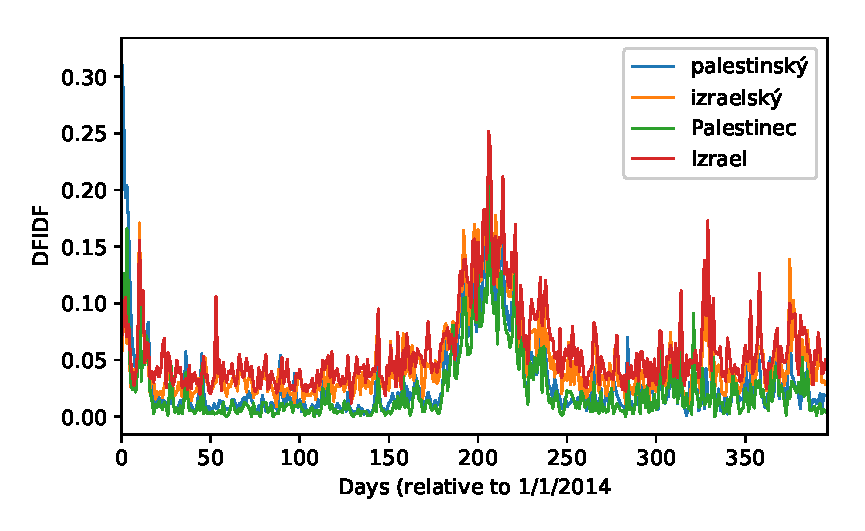
\includegraphics{original_event}  % original event
  \caption{Example of an event detected using the original method. The event consists of the words \textit{palestinian}, \textit{israeli}, \textit{Palestinian} and \textit{Israel}, respectively.}
  \label{fig:original-event}
\end{figure}


\section{Greedy approach}
In this section, we modify the original method to use the Word2Vec model to measure semantic similarity between words. Unlike the document overlap \eqref{eq:document-overlap}, this new similarity measure is able to distinguish semantically similar words even when they do not appear in the same documents. This may happen, for instance, when different authors each use distinct vocabulary when referring to the same event.


\subsection{Semantic similarity}
Some of the astounding results of the Word2Vec model arise from semantically similar words forming clusters \citep{linguistic-regularities} in terms of cosine similarity, which is a standard measure used in information retrieval \citep{information-retrieval, cosine-similarity}.

We replace the document overlap in the cost function \eqref{eq:cost-function-original} by cosine similarity between Word2Vec embeddings, though with a small modification. The cosine similarity is bounded in $[-1, 1]$ with -1 denoting the least degree of similarity. This means that the cost function would reach negative values for highly dissimilar words. This would be a problem, as Algorithm \ref{alg:greedy-event-detection} attempts to minimize it. Consequently, we will transform the cosine similarity into $[0, 1]$, just like the document overlap \eqref{eq:document-overlap}.

The similarity between a set of words $\featset$ and a word $w \notin \featset$ is defined as

\begin{equation}
	\semsim{\featset}{w} = \left( \frac{\inp[\big]{\bar{\embed}_{\featset}}{\embed_{w}}}{\| \bar{\embed}_{\featset} \| \cdot \| \embed_{w} \|} + 1 \right) /\ 2,
\end{equation}

where $\bar{\embed}_{\featset}$ is the mean of all vector embeddings of $\featset$ and $\embed_{w}$ is the vector embedding of $w$. Here, the mean vector virtually represents the central topic of words in $\featset$.


\subsection{Cost function}
We redefine the cost function \eqref{eq:cost-function-original} as

\begin{equation} \label{eq:cost-function}
	\cost{\featset}{w} = \frac{\text{Dist}( \featset \cup w )}{\semsim{\featset}{w} \cdot \sum_{u \in \featset \cup w}{\text{DPS}_{u}}},
\end{equation}

where $\text{Dist}(\cdot)$ is the original trajectory distance function \eqref{eq:trajectory-distance}.

In the original method, \cite{event-detection} defined the cost function \eqref{eq:cost-function-original} for a set of words. However, in Algorithm \ref{alg:greedy-event-detection}, it is always applied on a union of an event constructed so far, and a newly added word. The new cost function must now be applied on such event and word separately due to the nature of Word2Vec similarity definition.

Having constructed the cost function, we use Algorithm \ref{alg:greedy-event-detection} to detect events once again.


\begin{figure}[H]
  \centering
  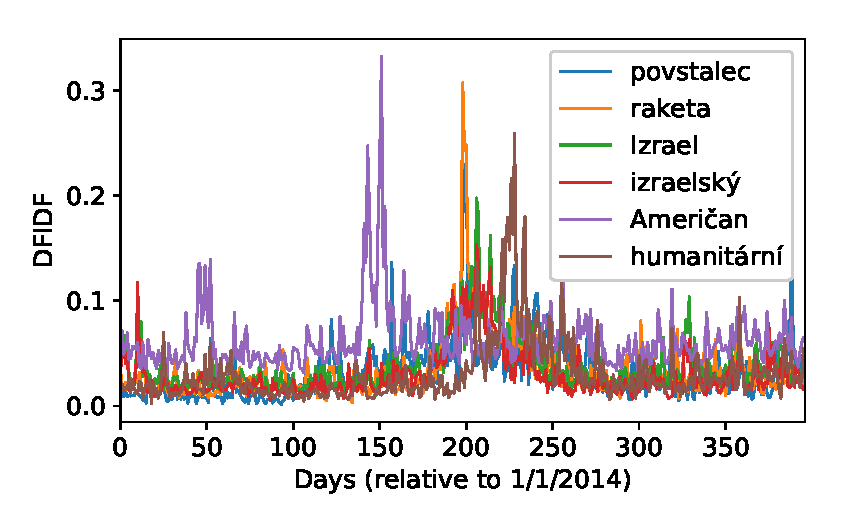
\includegraphics{greedy_event}  % greedy event
  \caption{Example of an event detected using the greedy method. The event consists of the words \textit{to shoot}, \textit{missile}, \textit{Israel} and \textit{israeli}, and is related to the same real event as \autoref{fig:original-event}.}
  \label{fig:greedy-event}
\end{figure}


\section{Cluster-based approach}
Realizing that the keyword-based event detection resembles word clustering, we decided to investigate this idea. In the final method, we apply a clustering algorithm equipped with a custom distance function to the set of eventful words. The distance function is actually a modification of the cost function yet again, though some means have to be taken to make it usable in this context. First, we need to consider a proper clustering algorithm.

The obvious requirement for the clustering algorithm is that it must require no prior knowledge of the desired number of clusters. Another requirement is that the algorithm must accept a custom distance measure.

We considered three candidate algorithms: Affinity propagation \citep{affinity-propagation}, DBSCAN \citep{dbscan} and its modification, HDBSCAN \citep{hdbscan}.

During our experimentation, Affinity propagation performed poorly, its clusters being often seemingly random and of low quality. The quality of HDBSCAN clusters was considerably better, though the algorithm took longer to converge as the number of eventful words grew. It also required to tune multiple parameters, which was difficult to do without any annotated data. We decided to use the DBSCAN algorithm, which outperformed Affinity propagation as well, and does not require to tune as many parameters as HDBSCAN.

In addition to the previously stated requirements, DBSCAN is also capable of filtering out noisy samples (in our case words), not fit for any of the clusters. This property will prove advantageous for our task, as will become clear during the evaluation in \autoref{sec:noise-evaluation}.


\subsection{Noise filtering}
Before we apply clustering, we filter out the noisy parts from the word trajectories. Most words are on some level reported all the time, though only a fraction of these reportings corresponds to notable events. Unlike the greedy optimization described previously, clustering is prone to such noise, and would yield clusters of poor quality, often with trajectories being put together only due to their noisy parts being similar. Additionaly, with DBSCAN capable of filtering out noisy samples, some high quality words could be discarded precisely due to this noise in their (otherwise eventful) trajectories.

We want to keep only those trajectory parts exceeding a certain frequency level, distinguishing notable bursts from the general noise. We do this by computing a cutoff value for each event trajectory and discarding the sectors falling under this cutoff. This procedure is adopted from \cite{online-search-queries}. The algorithm is based on computing a moving average along the trajectory, and works as follows:

\begin{algorithm}[H]
\begin{algorithmic}[1]
\caption{Burst filtering}
\label{alg:burst-filtering}
\Input $\text{window-length} \ l,\ \text{word trajectory} \ \vect{\traj_{w}}$

\State $\vect{MA}_{l} = \text{Moving Average of length} ~ l ~ \text{for} ~ \vect{\traj}_{w} = \left[ \traj_{w}(1), \traj_{w}(2), \dots, \traj_{w}(\streamlen) \right]$

\State $\mathit{cutoff} = \text{mean} \left( \vect{MA}_{l} \right) + \text{std} \left( \vect{MA}_{l} \right)$

\State $\vect{bursts}_{w} = \left[ \traj_{w}(t) \mid \traj_{w	}(t) > \mathit{cutoff} \right]$

\Output $\vect{bursts}_{w}$
\end{algorithmic}
\end{algorithm}


\subsection{Distance function}
We now define the distance function used by DBSCAN. It conveys similar information as the cost function in the previous two algorithms. We still need to measure the trajectory distance as well as semantic similarity between words, though the distance will now be defined strictly pairwise.

For a measure of trajectory distance, we replace the Kullback-Leibler divergence by the Jensen-Shannon divergence JSD \citep{js-divergence-1}, which is symmetric in its arguments. This is a necessary property of the distance function.

Although \cite{event-detection} did symmetrize the Kullback-Leibler divergence, they did not provide any source for their symmetrization form. We were unable to find a case where that particular form was used, though we discovered the Jensen-Shannon divergence, which comes from stronger mathematical background \citep{js-divergence-1, js-divergence-2}. It also tended to improve the clustering quality during our experimentation, as opposed to the original symmetrization. We then decided to replace the original paper's KL-divergence symmetrization by the JS-divergence.

Instead of semantic \textit{similarity}, we measure semantic \textit{distance} as the Euclidean distance between two word vector embeddings. The reason is that Euclidean distance is unbounded, which makes it possible for the samples to be spread farther apart. Since DBSCAN is a density-based clustering algorithm, having high density areas consisting of words with low trajectory distance and similar cosine similarities would cause them to appear in the same cluster. This would cluster the words only in terms of their trajectories, not semantics.

The distance between two words $v$ and $w$ with (normalized and filtered using Algorithm \ref{alg:burst-filtering}) trajectories $\vect{\trajn}_{v},\ \vect{\trajn}_{w}$ and Word2Vec embeddings $\embed_{v},\ \embed_{w}$ is now defined as

\begin{equation}
	\distfunc{v}{w} = \jsd{\vect{\trajn}_{v}}{\vect{\trajn}_{w}} \cdot \| \embed_{v} - \embed_{w}\|_{2},
\end{equation}

with $\jsd{\vect{p}}{\vect{q}} = \frac{1}{2} \left( \kl{\vect{p}}{\vect{m}} + \kl{\vect{q}}{\vect{m}} \right) ,\ \vect{m} = \frac{1}{2} \left( \vect{p} + \vect{q} \right)$.


\subsection{Event detection}
Now, we describe the cluster-based event detection algorithm, which is a direct application of the DBSCAN algorithm and consequent noise filtering.

\begin{algorithm}[H]
\begin{algorithmic}[1]
\caption{Cluster-based event detection}
\Input $\text{Word set EW obtained in \autoref{chap:word-analysis}, matrix } \trajmat \text{, word embeddings for EW}$

\State Precompute a distance matrix $\distmat \in \R^{\left\vert \text{EW} \right\vert \times \left\vert \text{EW} \right\vert}$ with $\distmat_{ij} = \distfunc{w_{i}}{w_{j}}$

\State Apply DBSCAN to $\distmat$, obtaining $k$ clusters and the noisy cluster

\ForEach{$(w, cluster) \in \text{DBSCAN.clusters}$}
	\If{$cluster \neq noise$}
		\State $e_{cluster} = e_{cluster} \cup w$
	\EndIf
\EndFor

\Output $\text{Events} ~ \{ e_{1}, e_{2}, \dots, e_{k} \}$
\end{algorithmic}
\end{algorithm}


\begin{figure}[H]
  \centering
  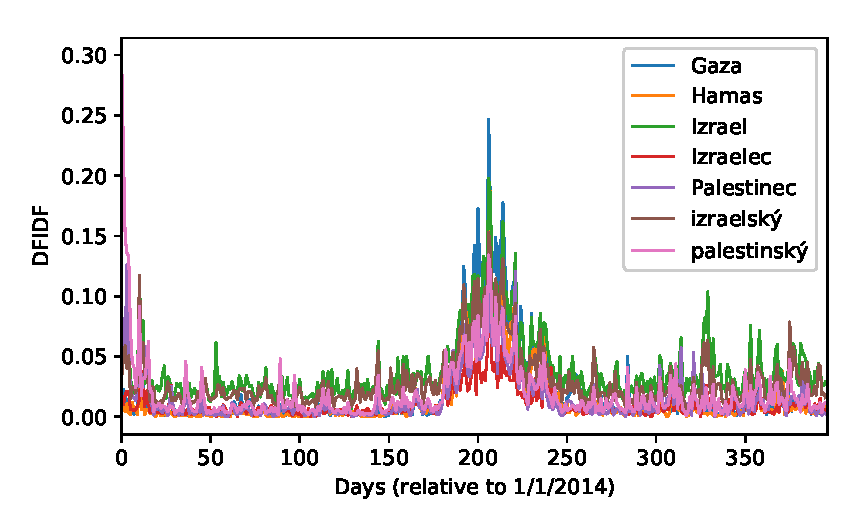
\includegraphics{cluster_event}  % cluster event
  \caption{Example of an event detected using the cluster-based method. The event is related to the same real event as \autoref{fig:original-event} and \autoref{fig:greedy-event}. Note that the trajectories are clear of noise due to application of Algorithm \ref{alg:burst-filtering}}
  \label{fig:cluster-event}
\end{figure}


\chapter{Document retrieval}
\label{chap:document-retrieval}
Having detected the events, we still have to present them to the user in a readable format. A set of keywords may be a concise representation for the computer, but it does not offer much insight into the event itself. We aim to generate short annotations for the events, based on which the user can decide to actually inspect the event more thoroughly and read some of the documents. Consequently, we need to retrieve some number of documents relevant to each event.

We can use each event's temporal and semantic information to query the document collection. The former is trivial -- simply select the documents published within an event's bursty period. The latter will prove more complicated, and we will need to employ some more information retrieval techniques to obtain semantically similar documents.

As of now, an event $e$ is described by a set of its keywords, $\kw{e}$. The goal is to convert this keyword representation to a document representation, $\doc{e}$ of documents related to $e$.

\section{Event burst detection}
First, we need to detect the period when the particular event occurred, so that we can retrieve the documents published around that time. We do this in five steps:

\begin{enumerate}
	\item Construct the event trajectory from the trajectories of its keywords.
	\item Clean the event trajectory.
	\item Determine the event's periodicity.
	\item Fit a probability density function to the event trajectory.
	\item Take the region(s) with the highest density as the bursty period(s).
\end{enumerate}


\subsection{Event trajectory construction}
We will first need to construct an \textit{event trajectory} out of its \textit{keyword trajectories}. We do this by computing a weighted average of the event's keyword trajectories, with weights being the keyword DPS. This ensures that less important words with slightly different time characteristic will not shift the trajectory away from the actual burst.

\begin{equation}
	\vect{\traj_{e}} \coloneqq \frac{1}{\sum_{k \in \kw{e}}{\text{DPS}_{k}}} \sum_{k \in \kw{e}}{\text{DPS}_{k} \cdot \vect{\traj}_{k}}
\end{equation}

{\color{red} TODO: Graph of event keyword trajectories and the weighted average}


\subsection{Trajectory filtering}

Now, a typical event (shown in {\color{red} TODO: Put a pretty picture here}) will usually have some number of dominant bursts corresponding to the period(s) when the event actually occurred. Additionally, there will be some milder, noisy bursts due to the keywords appearing elsewhere, independently of that particular event.

We aim to fit a probability density function to the event trajectory. However, the process would pointlessly try to fit the density to the noisy parts as well as to the bursts. Once again, we apply the Burst filtering algorithm described in \autoref{chap:event-detection} to filter out noise, this time from the event trajectories.

\subsection{Event periodicity}
We apply the signal processing techniques described in \autoref{chap:word-analysis} once more, this time to determine the dominant period $\text{DP}_{e}$ of each event $e$. After obtaining the periodogram, the dominant period is defined as the inverse of the frequency corresponding to the highest peak in the event trajectory:

\begin{equation}
	\text{DP}_{e} \coloneqq \frac{\streamlen}{\argmax\limits_{k \leq \ceil{\streamlen / 2}}{\|X_{k}\|^{2}}}.
\end{equation}

We then consider an event $e$ to be \textit{aperiodic} if it happened only once in the stream, that is if $\text{DP}_{e} > \ceil{\streamlen / 2}$. Similarly, the event is \textit{periodic} if $\text{DP}_{e} \leq \ceil{\streamlen / 2}$.

{\color{red} TODO: Graphs here}

\subsection{Density fitting}
We normalize the event trajectories to have unit sums, so they can be interpreted as probability distribution over days. An element $\traj_{e}(i)$ of the trajectory will denote a probability of that event occurring on day $i$. This allows us to fit a probability density function to them. \cite{event-detection} adapted a similar approach, though only for word rather than event trajectories.

We describe aperiodic and periodic events separately, as different probability distributions must be used in case of a single burst than in case of multiple bursts.

\begin{enumerate}

\item \textbf{Aperiodic events}

An aperiodic event trajectory $\vect{\traj}_{e}$ is modeled by a Gaussian distribution. We fit the Gaussian function

\begin{equation*}
	f(x) = \frac{1}{\sigma \sqrt{2 \pi}} \exp(-\frac{\left( x - \mu \right)^{2}}{2 \sigma^{2}})
\end{equation*}

to the trajectory $\vect{\traj}_{e}$. The parameters $\mu$ and $\sigma$ are estimated using non-linear least squares method. Unlike \cite{event-detection} who use the EM algorithm, least squares proved to be less prone to outliers, yielding a shape more resembling the actual trajectory.

\item \textbf{Periodic events}

A periodic event trajectory $\vect{\traj}_{e}$ is modeled using a mixture of $K = \floor{\streamlen / \text{DP}_{e}}$ Cauchy distributions (as many mixture components as there are periods), as in \cite{health-events}:

\begin{equation*}
	f(x) = \sum_{k = 1}^{K}{\alpha_{k} \frac{1}{\pi} \left( \frac{\gamma_{k}}{\left( x - \mu_{k} \right)^{2} + \gamma_{k}^{2}} \right)}
\end{equation*}

The mixing parameters $\alpha_{k} \geq 0,\ \sum_{k = 1}^{K}{\alpha_{k}} = 1$, location parameters $\mu_{k}$ and scale parameters $\gamma_{k}$ are estimated using the EM algorithm.

The Cauchy distribution has a narrower peak and thicker tails than the Gaussian distribution, which models the periodic bursts more closely. The individual bursts of a periodic event tend to be quite short, but even between two consecutive bursts, the frequency remains at a non-negligible level, which makes the Cauchy distribution a somewhat better choice.

\end{enumerate}


\subsection{Burst detection}
The bursty period of an aperiodic event $e$ is now defined as $\interval{\mu - \sigma}{\mu + \sigma}$. For a periodic event, there are $K = \floor{\streamlen / \text{DP}_{e}}$ bursty periods, each defined as $\interval{\mu_{k} - \gamma_{k}}{\mu_{k} + \gamma_{k}}$.

{\color{red} TODO: More graphs}


\section{Document retrieval}
We only describe the process for aperiodic events. The method is similar for periodic events, except applied on each burst individually.

We need to select some number of documents best representing an event $e$ out of all documents published within the event's bursty period. The only measure of semantics for an event we have is the event's keyword set $\kw{e}$. If we interpret $\kw{e}$ as a keyword query for the document collection, we arrive at the classical task of information retrieval.

In the original method by \cite{event-detection}, the task was simple due to the cost function used. In the paper, the only measure of semantic similarity used was the degree of document overlaps. That way, there was always at least one document in which all of the event's keywords appeared. This is not the case in our method, and we will need to measure the semantic similarity in a more sophisticated way.

There are a few approaches we could take, such as project all documents and queries to a TFIDF space \cite{information-retrieval} and sort the documents by their cosine similarity to the query. This simple approach does not go beyond a trivial keyword occurrence, though after applying some weighting scheme. We could enrich it using Latent Semantic Indexing \cite{lsi} to also take the document topics into account. This would however require us to ``train'' yet another model for this task only, which would be computationally and memory-intensive.

Instead, we decided to further utilize the trained word2vec model and use the recently introduced Word Mover's Distance \cite{wmd}.

The Word Mover's Distance (WMD) is a novel measure of document similarity based on word2vec embeddings of the document words. The similarity of two documents is measured as the minimum distance the word vectors of one document need to ``travel'' to reach the word vectors of the second document.

The WMD discards word order, which makes it suitable for our keyword queries. As the authors note, it achieves best results for short documents, in part due to the method being computationally expensive for larger pieces of text. Therefore, we apply the WMD on document headlines only.

Since the WMD is a measure of distance, we use the WMD similarity instead, defined as

\begin{equation}
	\wmdsim{d_{i}}{d_{j}} \coloneqq \frac{1}{1 + \wmd{d_{i}}{d_{j}}}
\end{equation}

\begin{algorithm}[H]
\begin{algorithmic}[1]
\caption{Document representation of an event}
\Input $\text{Event}\ e,\ \text{number of documents}\ n,\ \text{document stream}\ D$

\State $\mathit{burst\_docs} = \emptyset$

\ForEach{$\mathit{doc} \in D$}
	\If{$\mathit{doc.publication\_date} \in \mathit{e.burst}$}
		\State $\text{Compute}\ \wmdsim{\kw{e}}{\mathit{doc.headline}}$
		\State $\mathit{burst\_docs} = \mathit{burst\_docs} \cup \mathit{doc}$
	\EndIf
\EndFor

\State $\text{Sort}\ \mathit{burst\_docs}\ \text{by the computed}\ \text{Sim}_{\text{WMD}} \ \text{in descending order}$
\Output $\doc{e} = \text{first}\ n\ \text{elements of}\ \mathit{burst\_docs}$
\end{algorithmic}
\end{algorithm}

\chapter{Event annotation}
The final step of our method is to annotate the detected events in a human-readable way. We aim to generate short summaries so that the user does not have to process a large quantity of text, and can just skim through a few sentences to decide whether he is interested in that particular event. If so, then he can examine the event more closely and go through the actual documents, which we have retrieved in chapter \autoref{chap:document-retrieval}.

Although the keyword set discovered in \autoref{chap:event-detection} provides a concise representation of an event, it can lead to ambiguities or simply not reveal enough information. The keywords should be considered an internal representation used in the detection process, not a feature presentable to the user.

An example of such event whose background is unclear from the keyword set is shown in \autoref{fig:not-recognizable}. After manual examination, we discovered that the event concerns Viktor Yanukovych being ousted from Ukraine's presidency, though it is unclear from the keyword set.


\begin{figure}[H]
  \centering
  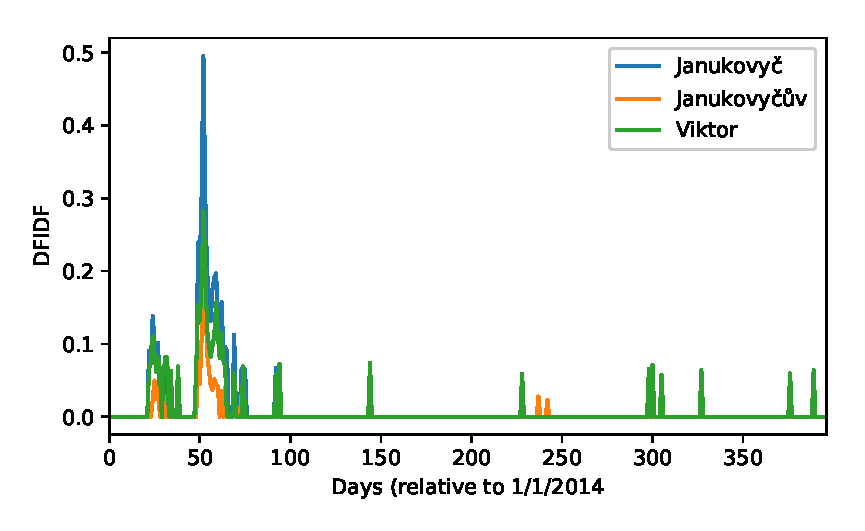
\includegraphics{18_words}  % event not recognizable from its keywords
  \caption{An event whose meaning is not clear from the keyword set.}
  \label{fig:not-recognizable}
\end{figure}


A simple method is to annotate an event by the headline of the most relevant document in terms of Word Mover's Similarity. This may give insight of the general topic of the particular event, but it is unlikely that a whole event will be well characterized by a single document. For this reason, we also investigate a more complex method.

To obtain richer annotations, we apply multi-document summarization techniques to generate a short summary of an event's document set. More specifically, we attempt to extract a subset of sentences out of the event documents, which cover the general topic of the event without providing redundant information. As the documents come from different sources and describe the events from different perspectives, the result will not generally be a continuous paragraph, but more of a set of characteristic sentences. Still, a longer piece of text will likely provide a better insight into an event than a single headline.

We examined the multi-document summarization system presented in \cite{multi-summarization-1, multi-summarization-2}. This system was later improved by \cite{mogren-1}, who evaluated the usage of different word embedding techniques for sentence similarity measures. Their work led to the system presented in \cite{mogren-2} which aggregates several different similarity measures to obtain a better quality summary. We adapt their system and combine together several measures of sentence similarity suitable for the event detection task.


\section{Multi-document summarization}
In \cite{multi-summarization-1}, the authors formulate the task of multi-document summarization as a constrained combinatorial optimization problem, where the goal is to retrieve a subset of sentences maximizing a monotone submodular function $\quality{\cdot}$ measuring the summary quality.

A submodular function $\quality{\cdot}$ on a set of sentences $U$ satisfies the property of \textit{diminishing returns}; that is, for $A \subseteq B \subseteq U \setminus \{ v \},\ \quality{A \cup \{ v \}} - \quality{A} \geq \quality{B \cup \{ v \}} - \quality{B},\ v \in U$. This has an intuitive interpretation for text summarization, namely that adding a sentence $v$ to a longer summary does not improve the summary as much as adding it to a smaller one. The reason is that the information carried by $v$ is likely already present in the longer summary.

Even though solving the task exactly is NP-hard, a greedy algorithm is guaranteed to find a solution only a constant factor off the optimum, as discussed by the authors.

The summary quality is measured in terms of how representative it is to the whole set (coverage) and how dissimilar the sentences are to each other (diversity). The constraints limit the summary to a reasonable length by bounding the total number of words.

In \cite{multi-summarization-1}, basic submodular functions to be used in multi-document summarization are described. In \cite{multi-summarization-2}, these functions are further developed to better capture the semantic properties of sentences.

Mathematically, the task is formulated as

\begin{equation}
\begin{alignedat}{-1}
\max_{S \subseteq U} & \quad \quality{S} = \coverage{S} + \lambda \diversity{S} \\
\text{s. t.} & \quad \sum_{i \in S}{\sentcost_{i}} \leq \budget,
\end{alignedat}
\end{equation}

where $U$ is the set of all sentences from the document set being summarized, $\sentcost_{i}$ is the number of words in sentence $i$ and $\budget$ is the total budget, i.e. the desired maximum summary length.

A feasible set $S$ maximizing $\quality{\cdot}$ will provide a reasonable number of sentences well capturing the overall topic of the whole document set, no two of which being redundant. What remains is to define the coverage function $\coverage{\cdot}$ and diversity function $\diversity{\cdot}$, whose influence can be controlled by the parameter $\lambda \geq 0$. Additionally, the functions must be defined in a way that the submodularity conditions from \cite{multi-summarization-1} are not violated, so that a greedy algorithm can still be used with performance guarantee.


\section{Coverage function}

In \cite{multi-summarization-2}, the coverage function $\coverage{\cdot}$ is defined in terms of pairwise sentence similarity $\semsim{\cdot}{\cdot}$ as

\begin{equation}
\coverage{S} = \sum_{i \in U}{\min{\Big\{ \sum_{j \in S}{\semsim{i}{j}}, \alpha \sum_{j \in U}{\semsim{i}{j}} \Big\} }}.
\end{equation}

The first argument of the minimum measures the similarity between the sentence $i$ and the summary $S$, while the second argument measures the similarity between the sentence $i$ and the rest of the sentences $U$. The number $\alpha \in [0,1]$ is a threshold coefficient controlling the influence of the overall similarity.

In \cite{multi-summarization-1}, the authors further prove that if $\semsim{i}{j} \in [0,1]\ \forall i, j \in U$, the whole function remains submodular.

Originally, only a simple cosine similarity between TFIDF sentence vectors \citep{information-retrieval} was used as $\semsim{\cdot}{\cdot}$. \cite{mogren-1} examined various methods of word embeddings to obtain a finer measure of similarity. This alone outperformed the original method. In \cite{mogren-2}, a more complex system aggregating multiple similarity measures was built, further improving the summary quality. The authors compute the sentence similarity $\semsim{i}{j}$ as a product of these individual similarities, all bounded in $[0, 1]$:

\begin{equation} \label{eq:aggregated-similarity}
	\semsim{i}{j} = \prod_{l}{\similarity_{s_{i}, s_{j}}^{l}}.
\end{equation}

We use this method with several different similarity measures fit for the event detection task. Next, we describe the individual sentence similarities used.

\subsection{TFIDF similarity}

The first measure used is the standard cosine similarity between TFIDF (Term Frequency-Inverse Document Frequency) vectors \citep{information-retrieval} of two sentences $s_{i}$ and $s_{j}$. Such method is a simple measure of document similarity often used in information retrieval.

If we denote the frequency of the word $w$ in sentence $s_{i}$ as $\text{tf}_{w,i}$ and the inverse document frequency of $w$ as $\text{idf}_{w}$, the similarity is written as

\begin{equation}
	\similarity_{s_{i}, s_{j}}^{\mathit{TFIDF}} = \frac{\sum_{w \in s_{i} \cup s_{j}} \text{tf}_{w,i} \cdot \text{tf}_{w,j} \cdot \text{idf}_{w}^{2}}{\sqrt{\sum_{w \in s_{i}} \text{tf}_{w, i}^{2} \cdot \text{idf}_{w}^{2}} \cdot \sqrt{\sum_{w \in s_{j}} \text{tf}_{w, j}^{2} \cdot \text{idf}_{w}^{2}}}.
\end{equation}

The term frequencies are always non-negative, and so the whole cosine similarity is in $[0, 1]$.

The major setback of TFIDF similarity is that it does not go beyond simple word overlap, though weighted to diminish stopwords and amplify important words. That means that if two sentences convey essentially the same information through different vocabulary, they will not be ranked similar due to having only a few words in common. That can be a problem in larger document collections from different sources and authors.

\subsection{Word2Vec similarity}

We attempt to solve this problem by considering the word embeddings of the individual words, as first examined by \cite{mogren-1}.

We represent a sentence $s_{i}$ by summing together the vector embeddings of its words, $\embed_{i} = \sum_{w \in s_{i}} \embed_{w}$. The similarity of two sentences is then the cosine similarity of these vectors, transformed to $[0, 1]$:

\begin{equation}
	\similarity_{s_{i}, s_{j}}^{\mathit{W2V}} = \left(\frac{\inp{\embed_{i}}{\embed_{j}}}{\| \embed_{i} \| \cdot \| \embed_{j} \|} + 1 \right) / \ 2.
\end{equation}

This similarity brings a finer distinction of word-level semantics. This means that even if two sources reporting the same event use fairly different vocabularies, the sentences will still be ranked similar.

\subsection{TR similarity}

The next measure uses Text Rank (TR) similarity, as defined by \cite{textrank}. Each sentence is represented by a set of words, and the overlap of these sets is measured. \cite{mogren-2} achieved best results by combining the TFIDF similarity, word embeddings and the TR similarity, which is defined as

\begin{equation}
	\similarity_{s_{i}, s_{j}}^{\mathit{TR}} = \frac{\left| s_{i} \cap s_{j} \right|}{\log{\left| s_{i} \right|} + \log{\left| s_{j} \right|}}.
\end{equation}


\subsection{Keyword similarity}

In addition to the three previously described similarities, \cite{mogren-2} considered a keyword similarity, which measures the overlap between two sentences and a predefined keyword set. Having previously obtained the event keyword representation $\kw{e}$, we use this measure to make sure the sentences actually concern the particular event.

The similarity is defined as 

\begin{equation}
	\similarity_{s_{i}, s_{j}}^{\mathit{KW}} = \frac{\sum_{w \in \left( s_{i} \cap s_{j} \cap \kw{e} \right)} \text{tf}_{w} \cdot \text{idf}_{w}}{\left| s_{i} \right| + \left| s_{j} \right|}.
\end{equation}

The measure effectively chooses only those sentences having non-zero word overlap with the keyword set. It also breaks the summary fluency, making the summary more of a set of sentences characteristic for the given event. On the other hand, the resulting sentences will be highly relevant to the event, often revealing important information about it.

This tradeoff between fluency and quality is more worth it when summarizing a large number of documents. Even without the keyword similarity, the chance that two summary sentences will make sense consecutively is quite small, when they come from different documents.

If an event consisted of only one or two documents, it would make sense to use a different measure to reach better fluency.

\section{Diversity function}
Now, we can define the diversity function, which will positively reward a summary consisting of non-redundant sentences. \cite{multi-summarization-2} first applied the K-Means clustering algorithm to the TFIDF vectors of the sentences in $U$. The diversity function then positively rewards summaries whose sentences come from different clusters. If the clustering well separates the sentences in the semantic sense, the sentences in different clusters will not carry redundant information.

The diversity function is defined as

\begin{equation} \label{eq:diversity}
	\diversity{S} = \sum_{k = 1}^{K} \sqrt{\sum_{j \in S \cap P_{k}} r_{j}},
\end{equation}

where $P_{k},\ k = 1, \dots, K$ is a clustering of the sentence set $U$. The value $r_{j} = \frac{1}{\left| U \right|} \sum_{i \in U} \similarity_{s_{i}, s_{j}}^{\mathit{TFIDF}}$ is the singleton reward for adding the sentence $i$ into the summary $S$.

This function positively rewards diverse sentences in a sense that once an element $i$ from a cluster $P_{k}$ is chosen, other elements from the same cluster will have diminishing gains due to the square root function (see \cite{multi-summarization-2} for a concrete example). The summarization will then prefer sentences from yet unused clusters.


\section{Optimization}
Having defined the cost function $\quality{\cdot}$, we can use the greedy algorithm defined in \cite{multi-summarization-1} to obtain the desired summary $\annot{e}$ for an event $e$.

For the experiments, we set a budget of 50 words. In the diversity function the number of clusters $K$ was set to $\frac{\left| U \right|}{10}$, putting 10 sentences into each cluster on average. As for the other parameters, we used the values from the original papers \citep{multi-summarization-1, multi-summarization-2}. Additionally, we need to specify which documents we will use for the summarization. In theory, there is no limit to the number of documents, though it would make sense to use only a few most-relevant documents. In \autoref{chap:evaluation}, we will limit the number of documents for efficiency reasons.

\section{Results}
In \autoref{tab:pretty}, we show the annotation for the event depicted in \autoref{fig:not-recognizable}. Though the keywords do not reveal much, the event's topic is fairly clear from the longer summary. We also include the headline of the most relevant document for comparison. In this case, the headline does not provide much insight into the event.

\hspace{\fill}

\begin{tabularx}{\linewidth}{l l} \toprule[1.5pt]
\bf Janukovyč, Janukovyčův, Viktor & \bf (Feb 15 - Mar 2, 2014) \\ \midrule
\multicolumn{2}{p{\linewidth}}{\bf Kdo stojí za Viktorem Janukovyčem?} \\
\multicolumn{2}{p{\linewidth}}{Kyjevská úřadovna prezidenta Viktora Janukovyče je bez stráží. Režim Viktora Janukovyče se zhroutil. Moc ukrajinského prezidenta Viktora Janukovyče se o víkendu zhroutila. Odvolaného ukrajinského prezidenta Viktora Janukovyče stíhá policie. ``Já , Viktor Janukovyč, se obracím na lid Ukrajiny.'' Svržený ukrajinský prezident Viktor Janukovyč se voleb zúčastnit nechce.} \\ \bottomrule[1.25pt]
\caption{Annotation for the event depicted in \autoref{fig:not-recognizable}} \label{tab:pretty}
\end{tabularx}

\hspace{\fill}

In \autoref{tab:ugly}, an event with highly redundant summary is shown. In this summarization, the diversity function \eqref{eq:diversity} failed to diminish similar sentences, and most of the summary simply repeats the same information. On the other hand, the most relevant document's headline represents the event very well, and would suffice to make sense of it.

\hspace{\fill}

\begin{tabularx}{\linewidth}{l l} \toprule[1.5pt]
\bf Adriano, Krnáčová, primátorka & \bf (Oct 12 - Dec 1, 2014) \\ \midrule
\multicolumn{2}{p{\linewidth}}{\bf Pražskou primátorkou bude Adriana Krnáčová z ANO} \\
\multicolumn{2}{p{\linewidth}}{Novou pražskou primátorkou bude Adriana Krnáčová. Primátorkou Prahy bude Adriana Krnáčová (ANO). Novou pražskou primátorkou bude Adriana Krnáčová z ANO. Novou pražskou primátorkou bude Adriana Krnáčová z ANO. Adriana Krnáčová je původem ze Slovenska. Pražskou primátorkou byla zvolena Adriana Krnáčová z hnutí ANO. Bratislavská rodačka Adriana Krnáčová je primátorkou Prahy.} \\ \bottomrule[1.25pt]
\caption{Example of a summary with high degree of redundancy.} \label{tab:ugly}
\end{tabularx}

\hspace{\fill}

Neither of the summaries is fluent enough to be read as an article. In both cases, the summaries resemble unordered sets of sentences, most of which give some insight into the underlying event. The user can stil gain some information from these summaries and consequently decide whether he is interested in the events enough to read the documents.

Further examples of the generated summaries can be found in \autoref{app:clusters-events}.

\chapter{Conclusion}
%\addcontentsline{toc}{chapter}{Conclusion}
We examined how event detection methods depending on keyword representation could be improved by considering word embedding models, namely the Word2Vec model \citep{word2vec}. We tried to augment an existing method by \cite{event-detection} to use a Word2Vec-based similarity function to match semantically related words together. This did not bring significant improvement -- although the detected events were richer and less redundant, a notable amount of noise appeared. This made the events hard to assign to their real world counterparts, as most of their keywords did not contribute to any underlying topic.

Then, we explored a different approach, where we interpreted the keyword-based event detection as a literal clustering task. We defined a custom distance function also utilizing the Word2Vec model as a semantic measure. We then applied a clustering algorithm equipped with this distance function to words previously selected as eventful. Our evaluation suggests that this method was more successful than both the original method and its Word2Vec modification. The resulting events were composed mostly of representative words and reached lesser redundancy and noisiness than the previous methods.

The disadvantage of both our methods is the necessity to train the Word2Vec model, which is time consuming. However, it can be trained once and than reused for subsequent detections, as long as the document vocabulary remains similar.

We also examined how the Word2Vec model could be used to retrieve documents concerning the detected events. We applied the Word Mover's Distance \citep{wmd} to documents within each event's bursty period as a measure of their relevance to that particular event's keyword set. We then selected the most relevant documents as the event's document representation. Although the documents were of high quality and represented the events well, the process took an unbearable amount of time. In the original method, the retrieval process was more straightforward and much more efficient.

Finally, we applied multi-document summarization techniques to the documents to obtain a short summary describing each event. This, along with the event's occurrence dates and document sets, are the outputs of our method presented to the user. The summaries serve the purpose of giving a quick reference of the event's topic, based on which the user may decide to examine the event further and go through the retrieved documents.

In future work, it would be beneficial to use a more efficient way of computing the documents relevant to each event. Traditional information retrieval techniques, such as Latent Semantic Indexing \citep{lsi} could be used here, perhaps with some domain specific knowledge of the underlying events, such as their bursty periods.

Also, we would like to examine how an event could be represented directly as a set of documents, rather than words. Although there are attempts to do so \citep{document-bursty-representation}, they require to fine-tune a number of parameters, and the document representation is again constructed using word trajectories. The Doc2Vec model \citep{doc2vec}, a generalization of Word2Vec able to embed whole documents in a vector space, could be used to obtain the semantic representation.

Instead of computing a cutoff value to clean a word or an event trajectory, as we did in \autoref{chap:event-detection}, further signal processing techniques could be applied on the trajectories to separate the dominant bursts from the underlying noise. The result would be a somewhat cleaner trajectory devoid of any milder bursts of no interest. This could lower the noisiness, since words would be matched together based on only the dominant activity, not any underlying influence, which still eludes the cutoff value method.


% Appendices
\appendix
\chapter{Appendix Title}
This is my appendix.


% Bibliography
\printbibliography

\end{document}